\chapter{Introduction}
\label{chapter:intro}

Stock markets have been a point of interest for researchers for a long time.
Stock market is a way for companies to obtain capital which they can invest into their own business.
In exchange, the person who invests into the companies stocks technically owns a piece of the company which can return profit to the investor two different ways.
The stock can grow in value, which allows the investor to sell the stock in higher price or the company itself can pay dividends to investors based on the number of stocks the investor owns from the company.

The price of the stock is simply determined by the law of supply and demand. 
If somebody is willing to pay a higher price for the stock then the price of the stock can grow.
Because of this the stock market is in continuous fluctuation where people are selling and buying the stocks with the price they think the stock is worth using stockbrokers as the middleman \cite{person}.
%All of this has lead to the question, how can we invest most optimally into stocks?
%This is where the following computational methods come in. 

When talking about stock analysis, people usually connect this with making profit the most optimal way.
However, stock analysis can be much more than this.
Because of the nature of stock market, where buyers define the actual price of the individual stock, stock market reflects a lot more information than one would think.
This hidden information can help us understand a lot of other phenomenoms that can influence stock market and this understanding can help us develop new innovations.

This reflected information also works the other way.
Information from other sources such as news and social media affect the stock market and both can be used to analyse it.
This is partly why the role of big data in stock data analysis has grown tremendously in the previous years.

Unfortunately, because of the monetary gains one can get from analysing stock data, publicly available information of the state of art stock analysis is quite hard to get.
This kind of information is usually kept private by companies that gain from them.
Innovating new ways to analyse stock is becoming harder and harder as breaking into the field needs more and more resources.

In this thesis, we try to alleviate the effort needed for novices start their learning process in this field and try to enable more smaller scale individuals to get in this field.
But first, in order to get a better understanding of how complex these systems can be, we are going to look stock analysis through a fictional but realistic application scenario.
We would like to note that, this thesis will be focusing only on the part of the depicted application, but the idea of the following section is to give the reader better overall view of the underlying domain.

%There are many strategies on how to invest into these stocks which depend on multiple factors such as; how much do you expect to profit with your investment, how much are you willing to take risk, do you want to make money by selling the stocks or by receiving dividends and so on.
%The underlying principle with every strategy is to minimize the risk you need to take in order to gain as much as profit as possible.
%Some of the strategies are based on subjective evaluation of the companies, but more technical strategies use metrics that are calculated from the financial statistics or the real-time market values.
%Strategies using the former data are called fundamental analysis and the strategies using latter data technical analysis.
%Neither of these approaches can predict the future of the market, but can statistically decrease the probability of larger losses in the market for the investor altough the probability of large losses is still not zero with these methods. \cite{fox}

%Fundamental analysis is based on the idea that each stock has a intrinsic value that can be larger than the actual price of the stock in the market and buying these will eventually lead to profits.\cite{sohnke}
%The fundamental analysis focuses on the financial metrics that consist of companys overall statistics.
%These are for example how much the company has made profit, how much the company has paid dividends and what is companys cash flow.
%These tell a lot about the growth of the company and how the future of the company looks like.
%These metrics are usually published quarterly four times a year and present more long-term statistics about the company.
%Because of this, the amount of data these values present is quite small in terms of space.

%The technical analysis that focuses on the real-time market values, on the other hand, needs new data almost daily.
%Stock exchanges are usually open from morning, opening around 8 to 10am, until evening, closing around 5 to 7pm on weekdays.
%Before and after this there are more limited pre- and after-hours trading which lasts usually around 1 to 2 hours depending on the exchange in which more limited stock trades can be made.
%During these hours multiple values are recorded on the prices of the stock from which the most important ones being: the highest price the stock was sold, the highest price the stock was sold and the number of stocks traded during the time interval.
%The technical analysis focuses on finding recognizable patterns through this data. \cite{murphy}
%Where the data used by the fundamental analysis was relatively small, these values can generate gigabytes of raw data in a week.

%Developing a system that can be used to conduct technical analysis means that the system should be planned to be able to handle large amounts of these data as time progresses.
%As such task is not trivial, the goal of this thesis is to provide developers and researchers, who want to analyse this data efficiently, basic knowledge and tools on what are the best current solutions on handling this data.
%With this knowledge these data scientists can save considerable amount of time without the need of trial and error when developing this kind of system from the ground up.

% for screenshots
\begin{figure}[ht]
    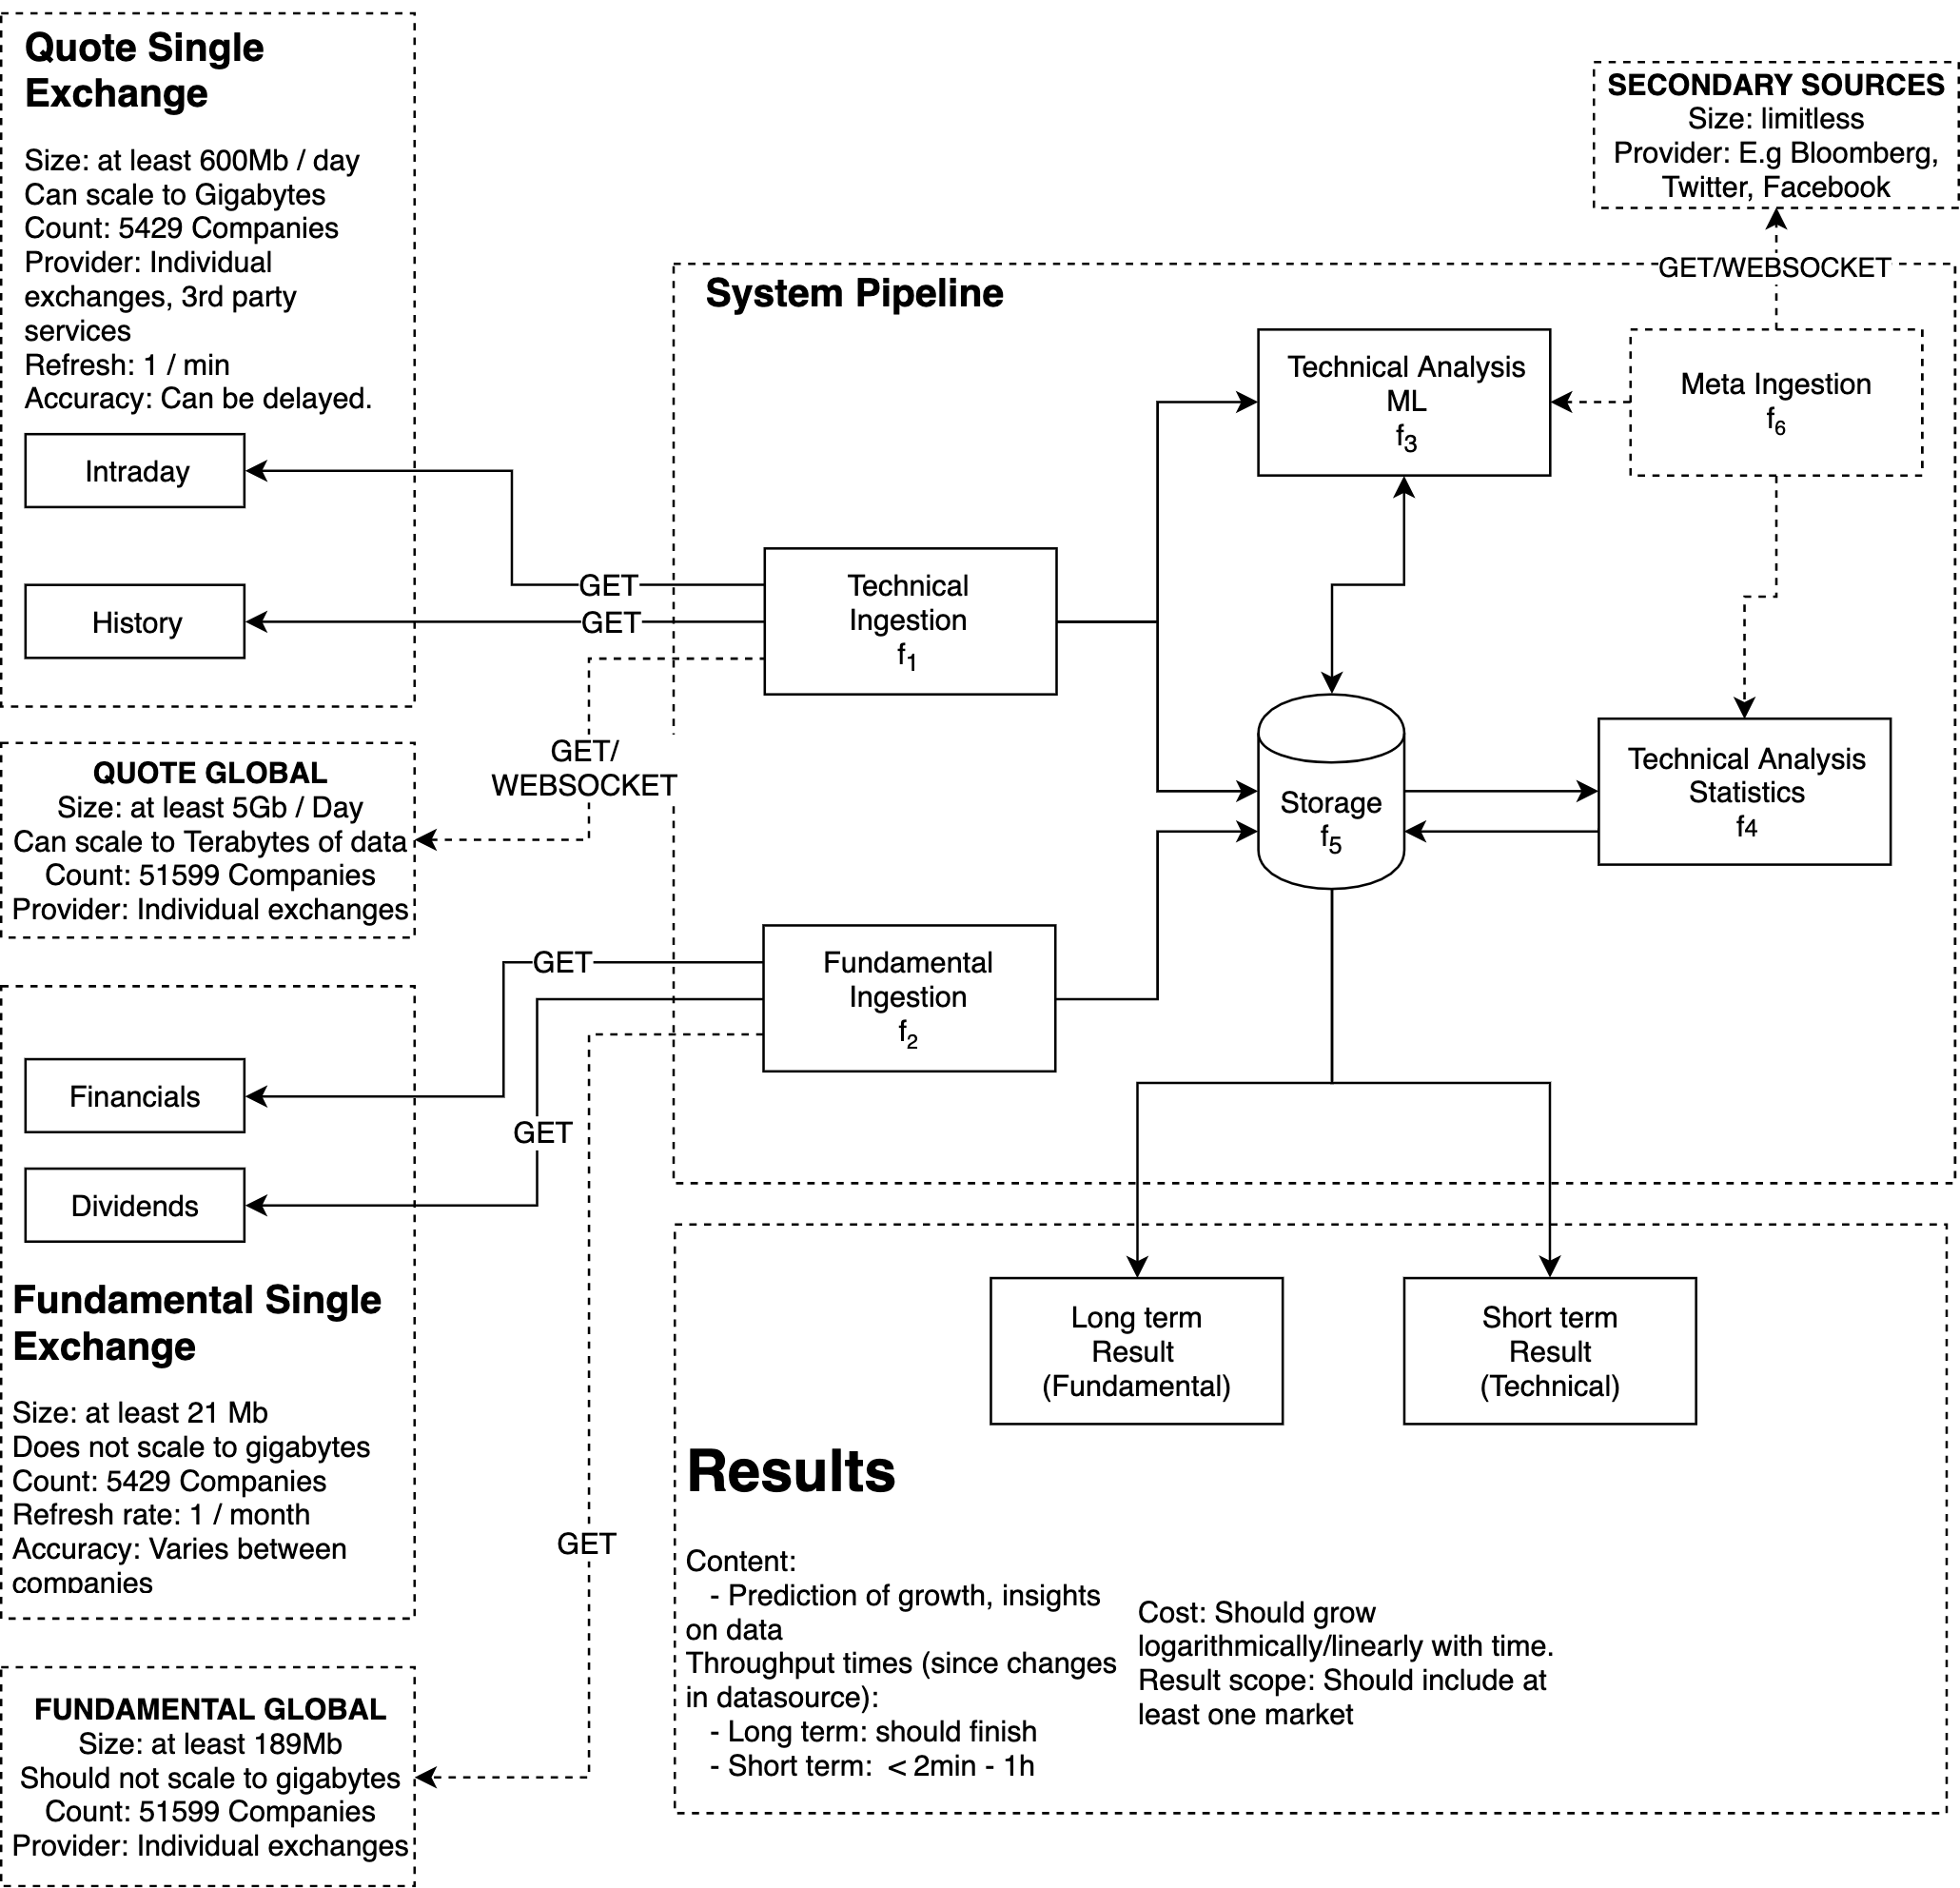
\includegraphics[scale=0.26]{images/system2} 
    \centering
    \caption{Example of a stock data pipeline}
\end{figure}

\section{Application scenario}
% research and engineering questions (why do you have to do it and why it is new)

In order to understand the system depicted above, we need to understand couple of key terms.
Stock analysis can be divided into two overlapping categories: fundamental analysis and technical analysis.
Fundamental analysis is based on the idea that each stock has an intrinsic value that can be larger than the actual price of the stock in the market and buying these will eventually lead to profits \cite{sohnke}.
Fundamental analysis is usually based on financial metrics and from a computational perspective the amount of data needed is not that large.
The technical analysis, on the other hand, focuses on the real-time market values and needs new data constantly.
This the kind of analysis where the amount of data can grow tremendously.
The technical analysis focuses on finding recognizable patterns through this data \cite{murphy}.

%To have a better picture what are the challenges of developing a system for technical analysis are, we will next look at a example case.
%The system we next
%This is to give the reader more complete view of a system that handles stock market data analysis.
%After this, for the rest of the thesis, we are going to focus on a part of this system, but the purpose of this example is to give a better view of the system as a whole in order to understand some of the requirements that these other components give to the focus of this thesis.

Somewhat normal system for analysing both fundamental and technical analysis is presented in Figure 1.1.
In the figure, the components marked with solid lines represent the core system functions, and the dashed lines represent add-on functionalities that should be possible to extend into the system in the future.
The requirements of the system are usually as follows;
The system should produce long ($r_1$) and short ($r_2$) term predictions of stock prices.
The computation of long term predictions can take time because of the nature of these predictions but the short term predictions should be between two minutes to one hour available.
Long term predictions are the result of fundamental analysis ($f_2$) and historical technical analysis ($f_4$) whereas the short term prediction should come mostly from quick technical analysis ($f_3$).
The cost of the system should grow logarithmically/linear with time meaning that the cost of processing and storing data should not exponentially increase over time.
Finally, the system should be able to fulfill these requirements for at least the +5000 companies in the major U.S stock markets which is the most accessible and individually significant market.

The data to the application can be ingested from two main types of data sources: quote and fundamental.
These sources consist of values that were briefly described previously in technical and fundamental analysis respectively.
The quote data is usually updated with minute intervals depending on the provider whereas the fundamental data does not change so often.
Theoretically, the fundamental data can change anytime, because of dividends which can be payed whenever the companies want but this does not happen often and these values are mostly used in the long term fundamental analysis so longer update intervals are acceptable.
In the Figure 1.1, these are separated into the single market ones ($d_1$ and $d_2$), which represent the minimum of at least including the U.S stock market and the other sources ($d_3$ and $d_4$) that provide the same data on other global markets.

In Figure 1.1, the extendable global data sources are grouped into one box but in reality this data would be ingested from numberable different providers as there is no single entity at the time of writing this that provides all of this data.
Theoretically the minimum of the maximum size of this extendable data would be 5Gb per day.
This is extrapolated in from the U.S market data based on statistics that in January 2019 there were globally 51 599 companies listed in the stock markets \cite{global}.
This amount can and will fluctuate as companies enter and exit the markets but it gives us the scale of data we are working with.

Today, stock market analysis has also a large focus on predicting stock prices using secondary data sources that can have reflect and affect the prices of stocks. 
These secondary data sources can be anything but at the moment one of the most researched sources are traditional media and social media data.
Examples of using this kind of data to predict predict stocks can be found in \cite{kao}, \cite{skuza} and \cite{wai}.
This is why the system should have the ability to extend to ingest data from arbitrary secondary sources ($f_6$ and $d_5$ in the Figure 1.1) to provide more versatile predictions about the stocks.
The amount of this data can be unlimited but is restricted to relevant sources.

Data is usually ingested from these data sources mainly using HTTP-protocol as this is the main method that these services ($d_1$ - $d_4$) provide.
Other possible methods that are usually available are, for example, Excel sheets and sometimes websockets, of which the websockets can be actually useful in cloud systems, but as the amount of data grows more custom file transfer methods are used.
However, as the HTTP-methods are currently the most publicly available technology, this thesis is going to focus on these.
The main ingestion functions are usually separated into two main types of functions $f_1$ and $f_2$. 
$f_1$ is constantly polling and processing data whereas $f_2$ handles batch processing.
Both of these function usually store their raw output into the storage, but $f_1$ passes this also to the immediate technical analysis.

The system should usually have two types of methods on analysing data.
For methods that allow streaming updates there is $f_3$, which can for example be cumulative/reinforced ML models and for methods that need historical data in order to calculate the prediction, there is $f_4$.
For fundamental analysis, there is no specific function as the introduced data sources usually provide these values pre-calculated and these values are usually easy to calculate dynamically with little to none amount of processing.

Finally, at the center of the system, there is the storage which is used to store the calculated predictions as well as the raw data from the data sources for later analysis.
For historical technical analysis, $f_4$, the storage should provide reasonable range query times when quering historical data and for the results the storage should provide efficient point queries for the results ($<$ 1s).

\section{Audience and Research Questions}

We saw the possible complexity of a stock data analysis pipeline in the previous section.
There are a lot of articles, such as \cite{adresic}, \cite{saha} and \cite{wenga}, about how to build a stock analysis pipeline but these usually are focused on the analysis of small amount of data in order to test some hypothesis.
Building a large-scale stock data analysis pipeline is a vastly complex task and to alleviate this process, this thesis plans to information on how to build one.

This thesis is aimed at novice data scientists that work or want to work with stock market data, but do not have any experience in big data technologies.
We define the term "novice" here to mean persons who have knowledge about analysing data using modern data analysis methods and know how to conduct this onto small datasets, but their proficiency lies strictly on the data analysis side.
This definition is not based on any existing literature and is only for clarity when we examine our target group.
This thesis could be useful for the reader because they have interest in the subject or are, for example, working for a startup which does not have resources to hire multiple persons with high degree on the subject.
This thesis is meant for this kind of people, as a place to find knowledge easily on how to get started.

As the system can be very complex as seen in the previous section, we will be focusing on the part of the pipeline that calculates models based on historical data.
This means the ingestion ($f_1$), storage ($f_5$) and analysis ($f_4$) of the historical data in a environment where the time restrictions are not that tight but the amount of data is enormous and the data can come from multiple different sources.
We have chosen this part of the pipeline as this is the part that has the highest probability to scale to big data first and is the part of the pipeline that is usually referred when talked about data analysis on stock market data.

The main goal of this thesis is going to be to make the data analysis in this big data context more accessible within the time constraints and resources that this thesis has.
What we mean by the word "accessible" here is that we want to minimize the time needed for the novice data scientist to start experimenting with their analysis, while making sure that developing models can continue smoothly in the future.
In this sense, things that make the process of analysing stock data in big data context "inaccesible" are things such as scattered information about options, outdated information online and lack of information on how to integrate different parts together.
This thesis plans to alleviate these aspects by providing aggregated information and an example case with solutions that can be used to navigate through these different problems.

%As the field of possible technologies is large, the main focus of this thesis would be the comparison of current relevant technologies in the context of stock data to help novice data scientists to decide what technologies to possibly use in their own projects.
%The main result of this thesis would be information and possible tools that developers could use to develop this kind of system more efficiently.
%Developers here can be people from companies that either do stock analysis as their main business or just want to analyze stock data efficiently.
%These results could also be used in research to implement analyzing pipelines more efficiently so that the research group can focus on the analyzing of the stock data instead of worrying with getting the data to these parts.

%Analyzing the stock data is also what most of the research today is focused on as this is the part that can actually produce profit.
%This means that most papers ignore the steps of ingesting and storing this data.
%Examples of this kind of papers are \cite{wu}, \cite{aghakhani} and \cite{kao}.
%So one of the goals of this thesis would be to bring more comprehensive picture of stock data pipelines. 

The research questions that this thesis tries to answer are: What is the current state of art in big data stock market analysis?, What makes stock analysis possibly inaccesible for novice data scientists? and How to build a pipeline that novice data scientist can use or benefit from?

For the first research question, we will be conducting a literary research on both academic and industrial stock market analysis using big data methods.
With the second research question, we want to understand what are the problems with the current environment for big data analytics on stock data for novice data scientists.
For this, we will be conducting literary study on the subject and we will analyse the results of this.

For the third and final research questions we will be building method that novice data scientists can use to build their own pipelines and we will analyze how this method works through a specific example case.
We will be focusing on the way the pipeline is build and what are the challenges that we face during it that could gravely affect novice data scientists.

%\section{Expected Outcome}

%For the first research question "What kind of pipelines are currently used?" this thesis plans to provide a study on currently used stock market analysis methods and used pipelines.
%The outcome will be a literature study on pipelines that are used in academia and industry based on public information.

%For the second question "How do these pipelines compare in the perspective of novice data scientist" the thesis would perform an analysis on the most promising big data pipeline technologies.
%This will be done in a form of comparison of different types of solutions that are either used in practice based on the results in the literature study for the first question or just seem promising for the use case.
%The result of this part could be used to decide what seems to be the most suitable technology to use to implement the stock analysis pipeline technically.

%For the last question "Which one is the best for novice data scientist as a starting point?" the thesis would implement open-source prototype solutions based on the results of the second research question.
%The expected outcome is to find a pipeline that a novice data scientist could develop onto which at the same time fulfills the aforementioned requirements.
%These prototypes could be used by anyone (company or individual) as it is or as a base to build a more complex system on top of them or use them as it is to perform data analysis.

\section{Structure of the Thesis}

We will start this thesis by examining the necessary background information in order to understand better the underlying domain and answer our first research question.
We will examine trends and state-of-art methods on stock analysis that have been used in recent scientific research.
Then we move on to examine what kind of pipelines exists in real-life.
We will be examining both commercial and research pipelines in order to give a more complete picture on options that exist.
We will also perform a literary research on technologies that are currently used to perform big-data ingestion, storing and analysis, selecting from the list of technologies mostly those that have been seen to be used in practice in this context while introducing couple of promising ones.

After this we move on to solve the second research question "What makes stock analysis possibly inaccesible?" and derive the requirements for our proposed method through this question.
We will define more precisely to whom this thesis is aimed at and examine what kind of challenges these people will face when starting big data analytics on stock market data.
Using this and the knowledge from the previous background chapter, we will derive the requirements for our method.

We will then define our key contribution that we think that would fulfill these requirements and present reasoning behind the choices we have made.
With this we will conclude the theoretical part of the thesis and start the empirical part.
In chapter 4.2, we will start by defining a special use case which we will be using to test this method in practice.
In the following chapters, we will report the process and end result of using this method.

After this we will move to analyse this test on what are the pros and cons on using this method in practice.
We will try our best to validate the claims that we make about the example case and try to bring up fair criticism that the end result could possibly have.
We then finish this chapter with a discussion on what could have been done better and how the systems developed could be improved in the future.
Then, to finish the thesis, we will have a conclusion chapter that summarizes the results of the thesis.

%We will then move on to focus on the last remaining research question. 
%In the first of these chapters we will be defining our proposed method of building a big data pipeline for stock analysis that is aimed at novice data scientists.
%We will reason why our method fulfills the requirements that we derived in the previous chapter and then move on to test this in practice.

%In the following chapter, we will describe what was done and what challenges we faced while implementing the systems.

%This chapter focuses mostly on the technical and practicalities that appeared during development.

%After this in the final real chapter we move on to analyse the results that we got from the implementation chapter. 
%We will try our best to validate the claims that we make about the example case and try to bring up fair criticism that the end result could possibly have.
%We then finish this chapter with a discussion on what could have been done better and how the systems developed could be improved in the future.
%Then finishing the thesis we will have a conclusion chapter that summarizes the results of the thesis.
